%%%%%%%%%%%%%%%%%%%%%%%%%%%%%%%%%%%%%%%%%
% Structured General Purpose Assignment
% LaTeX Template
%
% This template has been downloaded from:
% http://www.latextemplates.com
%
% Original author:
% Ted Pavlic (http://www.tedpavlic.com)
%
% Note:
% The \lipsum[#] commands throughout this template generate dummy text
% to fill the template out. These commands should all be removed when
% writing assignment content.
%
%%%%%%%%%%%%%%%%%%%%%%%%%%%%%%%%%%%%%%%%%

%----------------------------------------------------------------------------------------
%	PACKAGES AND OTHER DOCUMENT CONFIGURATIONS
%----------------------------------------------------------------------------------------

\documentclass{article}

\usepackage{fancyhdr} % Required for custom headers
\usepackage{lastpage} % Required to determine the last page for the footer
\usepackage{extramarks} % Required for headers and footers
\usepackage{graphicx} % Required to insert images
\usepackage{lipsum} % Used for inserting dummy 'Lorem ipsum' text into the template
\usepackage{enumerate}
\usepackage{booktabs}
\usepackage{amsmath}
\usepackage{subcaption}
\usepackage{tikz}
\usetikzlibrary{matrix}
\usepackage{algorithm2e}

\RestyleAlgo{boxruled}
\LinesNumbered

% Margins
\topmargin=-0.45in
\evensidemargin=0in
\oddsidemargin=0in
\textwidth=6.5in
\textheight=9.0in
\headsep=0.25in

\linespread{1.5} % Line spacing

% Set up the header and footer
\pagestyle{fancy}
\lhead{\hmwkAuthorName} % Top left header
\chead{\hmwkClass\ (\hmwkTitle)} % Top center header
%%\rhead{\firstxmark}
\rhead{} % Top right header
\lfoot{\lastxmark} % Bottom left footer
\cfoot{} % Bottom center footer
\rfoot{Page\ \thepage\ of\ \pageref{LastPage}} % Bottom right footer
\renewcommand\headrulewidth{0.4pt} % Size of the header rule
\renewcommand\footrulewidth{0.4pt} % Size of the footer rule

\setlength\parindent{0pt} % Removes all indentation from paragraphs

%----------------------------------------------------------------------------------------
%	DOCUMENT STRUCTURE COMMANDS
%	Skip this unless you know what you're doing
%----------------------------------------------------------------------------------------

% Header and footer for when a page split occurs within a problem environment
\newcommand{\enterProblemHeader}[1]{
\nobreak\extramarks{#1}{#1 continued on next page\ldots}\nobreak
\nobreak\extramarks{#1 (continued)}{#1 continued on next page\ldots}\nobreak
}

% Header and footer for when a page split occurs between problem environments
\newcommand{\exitProblemHeader}[1]{
\nobreak\extramarks{#1 (continued)}{#1 continued on next page\ldots}\nobreak
\nobreak\extramarks{#1}{}\nobreak
}

\setcounter{secnumdepth}{0} % Removes default section numbers
\newcounter{homeworkProblemCounter} % Creates a counter to keep track of the number of problems

\newcommand{\homeworkProblemName}{}
\newenvironment{homeworkProblem}[1][Problem \arabic{homeworkProblemCounter}]{ % Makes a new environment called homeworkProblem which takes 1 argument (custom name) but the default is "Problem #"
\stepcounter{homeworkProblemCounter} % Increase counter for number of problems
\renewcommand{\homeworkProblemName}{#1} % Assign \homeworkProblemName the name of the problem
\section{\homeworkProblemName} % Make a section in the document with the custom problem count
\enterProblemHeader{\homeworkProblemName} % Header and footer within the environment
}{
\exitProblemHeader{\homeworkProblemName} % Header and footer after the environment
}

\newcommand{\problemAnswer}[1]{ % Defines the problem answer command with the content as the only argument
\noindent\framebox[\columnwidth][c]{\begin{minipage}{0.98\columnwidth}#1\end{minipage}} % Makes the box around the problem answer and puts the content inside
}

\newcommand{\homeworkSectionName}{}
\newenvironment{homeworkSection}[1]{ % New environment for sections within homework problems, takes 1 argument - the name of the section
\renewcommand{\homeworkSectionName}{#1} % Assign \homeworkSectionName to the name of the section from the environment argument
\subsection{\homeworkSectionName} % Make a subsection with the custom name of the subsection
\enterProblemHeader{\homeworkProblemName\ [\homeworkSectionName]} % Header and footer within the environment
}{
\enterProblemHeader{\homeworkProblemName} % Header and footer after the environment
}

%----------------------------------------------------------------------------------------
%	NAME AND CLASS SECTION
%----------------------------------------------------------------------------------------

\newcommand{\hmwkTitle}{Homework\ \#6} % Assignment title
\newcommand{\hmwkDueDate}{Tuesday,\ March\ 13,\ 2018} % Due date
\newcommand{\hmwkClass}{FIN\ 513} % Course/class
\newcommand{\hmwkClassTime}{9:30am} % Class/lecture time
\newcommand{\hmwkAuthorName}{Wanbae Park} % Your name

%----------------------------------------------------------------------------------------
%	PARTIAL DERIVATIVES
%----------------------------------------------------------------------------------------
\newcommand{\pdv}[3][]{
	\frac{\partial^{#1}{#2}}{\partial{{#3}^{#1}}}
}

%----------------------------------------------------------------------------------------
%	EXPECTATION AND VARIANCE OPERATOR
%----------------------------------------------------------------------------------------
 \newcommand{\E}{\mathrm{E}}
 \newcommand{\Var}{\mathrm{Var}}
 \newcommand{\Cov}{\mathrm{Cov}}
 \newcommand{\Corr}{\mathrm{Corr}}

%----------------------------------------------------------------------------------------
%	TITLE PAGE
%----------------------------------------------------------------------------------------

\title{
\vspace{2in}
\textmd{\textbf{\hmwkClass:\ \hmwkTitle}}\\
\normalsize\vspace{0.1in}\small{Due\ on\ \hmwkDueDate}\\
\vspace{3in}
}

\author{\textbf{\hmwkAuthorName}}
\date{} % Insert date here if you want it to appear below your name

%----------------------------------------------------------------------------------------

\begin{document}


\maketitle

%----------------------------------------------------------------------------------------
%	TABLE OF CONTENTS
%----------------------------------------------------------------------------------------

%\setcounter{tocdepth}{1} % Uncomment this line if you don't want subsections listed in the ToC

%%\newpage
%%\tableofcontents
\newpage

%----------------------------------------------------------------------------------------
%	PROBLEM 1
%----------------------------------------------------------------------------------------

% To have just one problem per page, simply put a \clearpage after each problem

\begin{homeworkProblem}
	\begin{enumerate}[(a)]
		\item	%% Problem (a)
		Since yield-to-maturity is a discount rate which discount ``promised''
		payoff to current price, $F$ is represented as $F = \frac{1}{1 + y}$.
		\item	%% Problem (b)
		Under risk-neutral measure, all expected return is risk-free.
		Therefore, $F$ is represented as $F = \frac{p \times 1 + (1 - p) \times 0}{1 + R} = \frac{p}{1 + R}$.
		\item	%% Problem (c)
		Since expected return of the bond is $e$, and there is true survival probability $\pi$,
		$F$ is represented as $F = \frac{\pi \times 1 + (1 - \pi) \times 0}{1 + e} = \frac{\pi}{1 + e}$.
		\item	%% Problem (d)
		Since $F = \frac{p}{1 + R} = \frac{\pi}{1 + e}$, $\frac{\pi}{p} = \frac{1 + R}{1 + e}$.
		Furthermore, because the bond is risky, $e$ must be greater than $R$,
		therefore the inequality $\frac{\pi}{p} = \frac{1 + R}{1 + e} < 1$ holds.
		\item	%% Problem (e)
		From (d), risk-neutral survival probability is always greater than
		true survival probability. Since given true probability is 97\% and it is almost 100\%,
		risk-neutral survival probability might be 100\%. It means that under risk-neutral measure,
		expected payoff of bond is almost equal to 1. Therefore, yield-to-maturity is almost same as risk-free rate,
		and the bond price is almost equal to face value discounted at risk-free rate.
		Furthermore, since expected return of asset is 12\%, and firm's asset is not risk-free,
		risk-free rate must be less than 12\%. Therefore, bond price must le larger than $\frac{1}{1.12}$.
	\end{enumerate}
\end{homeworkProblem}

%----------------------------------------------------------------------------------------
%	PROBLEM 2
%----------------------------------------------------------------------------------------

\begin{homeworkProblem}
	Under Merton model, stock price is considered as a call option of firm value,
	with strike price is face value of a debt. Therefore, stock volatility can be calculated as follows.
	\begin{equation*}
		\begin{aligned}
			&S = VN(d_1) - Fe^{-r(T - t)}N(d_2)	\\
			&\pdv{S}{V} = N(d_1) ~~ \text{which is delta of call option.}	\\
			&\Rightarrow stock~volatility = N(d_1) \frac{V}{VN(d_1) - Fe^{-r(T - t)}N(d_2)} \sigma_V	\\
			&\text{where}~~d_1 = \frac{\log(V/F) + (r + \frac{1}{2}\sigma_V^2)(T - t)}{\sigma_V \sqrt{T - t}}
						d_2 = d_1 - \sigma_V \sqrt{T - t}	\\
						&F: \text{Face value of debt}
		\end{aligned}
	\end{equation*}
	By using the formula, stock volatilities were calculated with respect to
	stock prices from 0 to 40. The range of stock prices corresponds to
	the range of firm value from 11 to 110. Figure \ref{fig:prob2-stock volatility under Merton Model}
	shows the stock volatility as a function of stock price.
%----------------------------------------------------------------------------------------
	%% VOLATILITY ON MERTON MODEL
	\begin{figure}[ht]
		\centering
		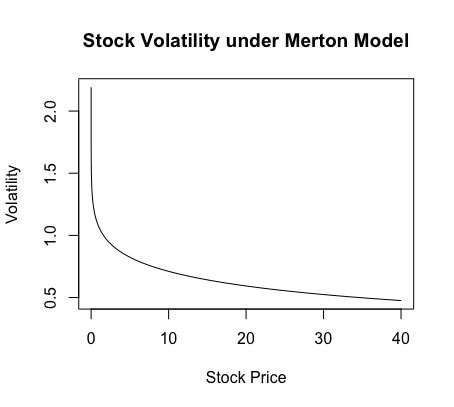
\includegraphics[scale = 0.6]{HW6_prob2_merton.png}
		\caption{Stock Volatility under Merton Model}
		\label{fig:prob2-stock volatility under Merton Model}
	\end{figure}
%----------------------------------------------------------------------------------------
	As shown in figure, stock volatility decreases as stock price increases.
	Furthermore, under constant elasticity of variance model(CEV Model),
	since stock price process is defined as $\frac{dS}{S} = \mu dt + \frac{\omega}{\sqrt{S}}dW$,
	the corresponding variance of stock price is $\frac{\omega}{\sqrt{S}}$.
	Figure \ref{fig:prob2-stock volatility under CEV Model} shows volatility
	as a function of stock price under CEV model.
%----------------------------------------------------------------------------------------
	%% VOLATILITY ON CEV MODEL
	\begin{figure}[ht]
		\centering
		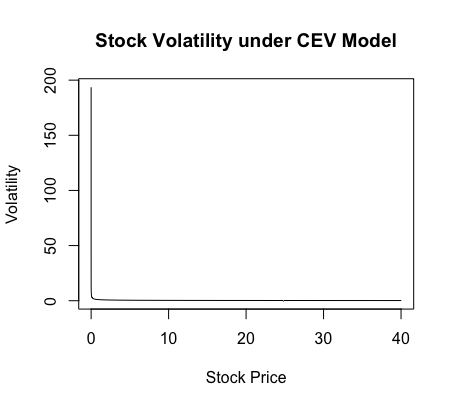
\includegraphics[scale = 0.6]{HW6_prob2_cev.png}
		\caption{Stock Volatilty under CEV Model}
		\label{fig:prob2-stock volatility under CEV Model}
	\end{figure}
%----------------------------------------------------------------------------------------
	As shown in figure, volatility also has a decreasing feature as stock price
	increases. However, since there is stock price in denominator term,
	if stock price gets closer to zero, volatility increases sharply.
\end{homeworkProblem}

%----------------------------------------------------------------------------------------
%	PROBLEM 3
%----------------------------------------------------------------------------------------
\begin{homeworkProblem}
	\begin{enumerate}[(a)]
		\item	%% Problem (a)
		Using the formula in question 2, volatilty multiplier was calculated
		for each volatility and face value.
		Figure \ref{fig:prob2-Volatility multiplier-fv=100} and
		\ref{fig:prob2-Volatility multiplier-fv=50} show volatilty multiplier
		with each face value with respect to volatility of firm value.
%----------------------------------------------------------------------------------------
		%% VOLATILITY MULTIPLIER WITH FACE VALUE 100
		\begin{figure}[ht]
			\centering
			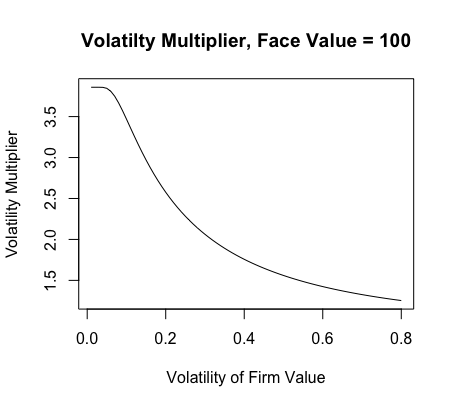
\includegraphics[scale = 0.6]{HW6_prob3_fv100.png}
			\caption{Volatility multiplier with face value 100}
			\label{fig:prob2-Volatility multiplier-fv=100}
		\end{figure}
%----------------------------------------------------------------------------------------
	%% VOLATILITY MULTIPLIER WITH FACE VALUE 50
		\begin{figure}[ht]
			\centering
			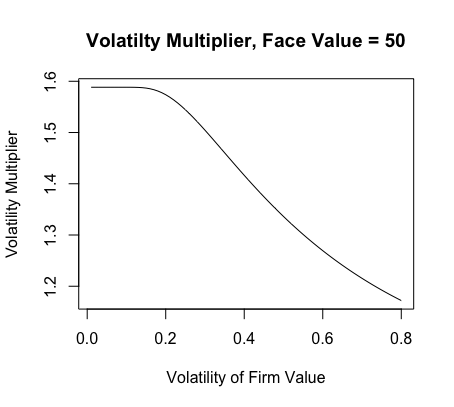
\includegraphics[scale = 0.6]{HW6_prob3_fv50.png}
			\caption{Volatility multiplier with face value 50}
			\label{fig:prob2-Volatility multiplier-fv=50}
		\end{figure}
%----------------------------------------------------------------------------------------
		As shown in figure, volatility multiplier remains constant if
		volatility of firm value is low, but as volatility of firm value
		increases, volatility multiplier starts to decrease after a threshold
		at some level.
		It means that after the level, marginal increase of stock volatility
		becomes less than the amount of increases in volatilty of firm value.
		Moreover, it can be found that the level of threshold is higher when
		face value of debt is lower, and volatility multiplier is higher when
		face value of debt is higher.
		\item	%% Problem (b)
		If idiosyncratic risk is added, then $\sigma_V$ increases, but
		$\pi_V$ does not increase. Therefore, $\pi_S = \pi_V \frac{\sigma_S}{\sigma_V}$
		decreases since volatility multiplier decreases as $\sigma_V$ increases,
		and $\pi_V$ remains constant. If $\sigma_V$ is low, changes in excess return of stock
		would not be too much because volatilty multiplier seems almost constant
		if $\sigma_V$ is less than threshold level.
		\item	%% Problem (c)
		From answer to (b), excess return of stock decreases as idiosyncratic risk
		in firm value increases. From firm's perspective, less cost of equity capital
		is better to sell equity in future. Therefore, managers will prefer to
		increase idiosyncratic risk in firm value.
	\end{enumerate}
\end{homeworkProblem}

%----------------------------------------------------------------------------------------
%	PROBLEM 4
%----------------------------------------------------------------------------------------
\begin{homeworkProblem}
	\begin{enumerate}[(a)]
		\item	%% Problem (a)
		Under Leland model, the optimal bankruptcy covenant is derived as
		$V_B = \frac{X}{1+X} \frac{\Gamma}{r} (1 - \Omega)$, where $X = \frac{2r}{\sigma^2}$.
		From this result, we can analyze comparative statics of the Leland model.
		\begin{enumerate}[(i)]
			\item	%% Problem (i)
			From the equation above, it can be showed that higher tax rate makes
			$V_B$ lower since all other parameter is positive.
			\item	%% Problem (ii)
			In order to investigate the effect of changes in risk-free rate,
			we can differentiate $V_B$ with respect to risk-free rate, $r$.
			\begin{equation*}
				\begin{aligned}
					V_B 	&= \frac{X}{1+X} \frac{\Gamma}{r} (1 - \Omega)	\\
							&= \Gamma (1 - \Omega) \frac{2r / \sigma^2}{1 + 2r / \sigma^2} \frac{1}{r}	\\
							&= 2(1 - \Omega) \Gamma \frac{1}{\sigma^2 + 2r}	\\
					\Rightarrow \frac{dV_B}{dr} &= 2(1 - \Omega) \Gamma \times (-\frac{1}{(\sigma^2 + 2r)^2} \times 2)	\\
							&= -4(1 - \Omega) \Gamma \frac{1}{(\sigma^2 + 2r)^2} < 0
				\end{aligned}
			\end{equation*}
			Therefore, higher risk-free rate makes optimal covenant level lower.
			\item	%% Problem (iii)
			The optimal covenant level does not include bankruptcy cost.
			It means that $V_B$ is independent of bankruptcy cost, $\alpha$.
		\end{enumerate}
		\item	% Problem (b)
		Assuming that manager of each country choose optimal coupon in order to
		maximize firm's equity value. Under Leland model, equity value is represented as
		$S = V_0 - (F - F^{TS} + F^{BC})$, where $F, F^{TS}, F^{BC}$ denotes
		value of debt, tax shield, bankruptcy cost, respectively. Plug the equation
		(5), (6), (7) in lecture note to the equation above, firm's stock price is calculated as follows.
		\begin{equation*}
			\begin{aligned}
				S 	&= V_0 - \left(\frac{\Gamma}{r} + \left[(1 - \alpha)V_B - \frac{\Gamma}{r}\right] \left(\frac{V_B}{V_0} \right)^X
						- \Omega \frac{\Gamma}{r} \left[1 - \left(\frac{V_B}{V} \right)^X \right]
						+ \frac{\alpha}{V^X} V_B^{1 + X} \right)	\\
					&= V_0 - \left(\frac{\Gamma}{r} + \left[V_B - \frac{\Gamma}{r}\right] \left(\frac{V_B}{V_0} \right)^X
							- \Omega \frac{\Gamma}{r} \left[1 - \left(\frac{V_B}{V} \right)^X \right]
						 \right)
			\end{aligned}
		\end{equation*}
		From the equation above, we can find that stock price is independent of bankruptcy cost.
		Therefore, regardless of choice in $\Gamma$, covenant level does not changes as bankruptcy cost changes,
		if others are constant.
	\end{enumerate}
\end{homeworkProblem}
\end{document}
